\documentclass[11pt]{beamer}

%%%%%%%% tema e cor %%%%%%%%
\mode<presentation> {
\usetheme{Dresden} % Raphael
%\usetheme{Darmstadt}
%\usetheme{Frankfurt} % Raphael
%\usetheme{Berlin}
%\usetheme{Madrid} % Rubens
%\usecolortheme{albatross}
}

\usepackage[brazil]{babel}
\usepackage[utf8]{inputenc}
\usepackage{graphicx} 
\usepackage{booktabs} 



\institute[UEA] 
{
%================= logo no meio =====================
\vspace*{-0.35cm}

\includegraphics[width=1.6cm]{img/logo-uea.png}
\vspace*{0.5cm}\\
Curso de Engenharia de Controle e Automação \\
Escola Superior de Tecnologia -- EST\\
Universidade do Estado do Amazonas -- UEA\\
\vspace{0.1cm}
Orientador: Israel Mazaira Morales
%\medskip
%\texttt{\{lods.eng,ronety\}@uea.edu.br} % emails
}
\date{\today}

\AtBeginSection[]
{
\begin{frame}
\frametitle{Conteúdo}
\tableofcontents[currentsection]
\end{frame}
}

%%%%%%%% titulo e subtitulo %%%%%%%%
\title[Trabalho de Conclusão de Curso]{Projeto de um Sistema de Abastecimento Pluvial Baseado em \textit{IoT}} 

%%%%%%%% nome dos autores %%%%%%%%
\author[Nunes, de S. R.]{Raphael de Souza Nunes} 

\begin{document}
\begin{frame}
\titlepage 

\end{frame}

\begin{frame}
\frametitle{Conteúdo} 
\tableofcontents 
\end{frame}

%%%%%%%% slides %%%%%%%%
\section{Introdução} 
\begin{frame}{Introdução}
\begin{itemize}
\item Nos últimos anos, crises relacionadas ao abastecimento e à qualidade da água potável têm sido observadas em todo o Globo;
\item A região norte, possuindo a maior reserva de água potável do Brasil e também os maiores índices de precipitação, é a região que possui as taxas mais altas de desperdício \cite{globo};
\item O desperdício pode ser encontrado no ambiente doméstico e nas várias etapas de: coleta, armazenamento, processamento e principalmente na distribuição do recurso;
\end{itemize}
\end{frame}

\begin{frame}{Olá}
    Olá, tudo bem?
\end{frame}

\section{Justificativa}
\begin{frame}{Justificativa: blocos}
\begin{block}{Block 1}
Lorem ipsum dolor sit amet, consectetur adipiscing elit. Integer lectus nisl, ultricies in feugiat rutrum, porttitor sit amet augue. Aliquam ut tortor mauris. Sed volutpat ante purus, quis accumsan dolor.
\end{block}

\begin{block}{Block 2}
Pellentesque sed tellus purus. Class aptent taciti sociosqu ad litora torquent per conubia nostra, per inceptos himenaeos. Vestibulum quis magna at risus dictum tempor eu vitae velit.
\end{block}

\end{frame}

\section{Objetivos}
\begin{frame}{Objetivos}
\begin{block}{Objetivo Geral}
    O objetivo desse trabalho de conclusão de curso é a elaboração de um projeto base para aplicação de um sistema automatizado de coleta, armazenamento e distribuição de água da chuva com base em uma cisterna pluvial. Realizando medições de volume, através de sensores, acionamento de válvulas solenoides e motobombas por meio de comandos via interfaces \textit{desktop} e \textit{mobile}.
\end{block}
\end{frame}

\begin{frame}{Objetivos}
\begin{block}{Objetivos Específicos}
\begin{itemize}
    \item [(a)] Elaborar um módulo denominado \textbf{CCM - \textit{Cistern Control Module}} para aplicação no reservatório principal, realizando medições de nível, acionamento de \textit{motobomba}, direcionamento do fluxo de água em conexão com outros dispositivos via tecnologia \textit{Wi-Fi};
	\item [(b)] Elaborar um módulo denominado \textbf{TCM - \textit{Tank Control Module}} para aplicação no reservatório auxiliar, realizando medições de nível, direcionamento do fluxo de água em conexão com outros dispositivos via tecnologia \textit{Wi-Fi};
	\item [(c)] Elaborar um aplicação \textit{Android Mobile} (denominada \textbf{RCS APP}) e \textit{Desktop} (denominada \textbf{RCS DESKTOP}) para executar as ações: ativação e desativação de uma bomba d'água, direcionamento do fluxo de água, visualização de dados provenientes de sensores e estruturando a possibilidade de definir as condições que executem rotinas de acionamento automático;
\end{itemize}
\end{block}
\end{frame}

\begin{frame}{Objetivos}
    \begin{block}{Objetivos Específicos}
    \begin{itemize}
        \item [(d)] Configurar um sistema operacional embarcado conciso (baseado em \textit{kernel Linux}) aplicando-o a um microprocessador. O dispositivo deve possuir conexão com a \textit{Intranet} e servir como uma central de controle e armazenamento de dados, bem como ser hospedeiro do serviço de \textit{Broker MQTT};
        \item [(e)] Incluir no sistema, rotinas de leitura de sensores e acionamento de motobombas;
        \item [(f)] Organizar um repositório \textit{online} para realização de futuras atualizações (\textit{upgrades}) do \textit{firmware} embarcado.
    \end{itemize}
    \end{block}
\end{frame}


\section{Fundamentação Teórica}
\begin{frame}{Fundamentação Teórica}
\begin{itemize}
    \item Nós utilizamos essa abordagem
    \item Assim assim
    \item Assado
\end{itemize}
    
\end{frame}

\begin{frame}{Elementos Base}{Redes \textit{Wireless}}
      
\begin{itemize}
    \item O termo \textit{Wireless} provém do inglês: \textit{wire} (fio, cabo); less (sem);
    \medskip
    \item Possui vantagens cruciais para a aplicação do conceito de Internet das Coisas:
\end{itemize}    

\end{frame}

\begin{frame}{Elementos Base}{Redes \textit{Wireless}}
      
    \begin{itemize}
        \item \textbf{Maior produtividade - } disponibiliza acesso à rede em todo o raio de alcance onde o ponto de acesso está instalado, oferecendo liberdade de deslocamento com conexão contínua;
	
        \item \textbf{Flexibilidade de instalação -} podem ser instaladas em locais com temperaturas elevadas, em que os cabos não suportariam, ou em locais que necessitam de acesso temporário;
        
        \item \textbf{Redução de custo - } reduzem os custos de instalação, dispensando o uso de material para cada ponto de conexão;
        
        \item \textbf{Interoperabilidade e segurança - } capaz de comunicar sistemas de forma confiável e com segurança, possuindo chaves de acesso e até mesmo transferindo mensagens criptografadas.   
    \end{itemize}    
    
\end{frame}

\begin{frame}{Elementos Base}{Redes \textit{Wireless}}
    A topologia de uma rede IEEE 802.11 (\textit{Wi-Fi})  possui os seguintes elementos-chave:

    \begin{itemize}
        \item \textbf{BSS - \textit{Basic Service Set} -} corresponde a uma célula de comunicação \textit{wireless};
        \item \textbf{STA - \textit{Stations} -} são as estações de trabalho que comunicam-se entre si dendo da \textbf{BSS};
        \item \textbf{AP - \textit{Access Point} -} coordena a comunicação entre as \textbf{STA's} dentro da \textbf{BSS}. Na maioria das vezes roteadores realizam tal operação;
        
    \end{itemize}
    
\end{frame}

\begin{frame}{Elementos Base}{Redes \textit{Wireless}}
    \begin{itemize}
    \item \textbf{\textit{Bridge} -} faz a ligação entre diferentes redes, por exemplo, uma rede sem fio para uma rede cabeada convencional;
	\item  \textbf{ESS - \textit{Estended Service Set} -} consiste de várias células \textbf{BSS's} vizinhas que se interceptam e cujos \textbf{AP's} estão conectados a uma mesma rede tradicional. Nestas condições uma \textbf{STA} pode movimentar-se de um \textbf{BSS} para outr, permanecendo conectada à rede. Este processo é denominado \textit{Roaming}.
	\end{itemize}
\end{frame}

\begin{frame}{Elementos Base}{A Internet das Coisas}
    \begin{itemize}
        \item Um conjunto de tecnologias e protocolos associados que permitem que objetos se conectem a uma rede de comunicações e onde são identificados e controlados;
        \item Esse termo se tornou possível graças aos avanços tecnológicos e as reduções de custo de todos os dispositivos eletroeletrônicos, os quais possuem a capacidade de comunicação principalmente por meio de protocolos \textit{Wiress};
    \end{itemize}
    
\end{frame}

\begin{frame}{Elementos Base}{A Internet das Coisas}

    \begin{figure}
        \centering
        \caption{Protocolos utilizados para aplicacão do \textit{IoT} com base nos conceitos de redes. Relação entre velocidade-força e distância.}
        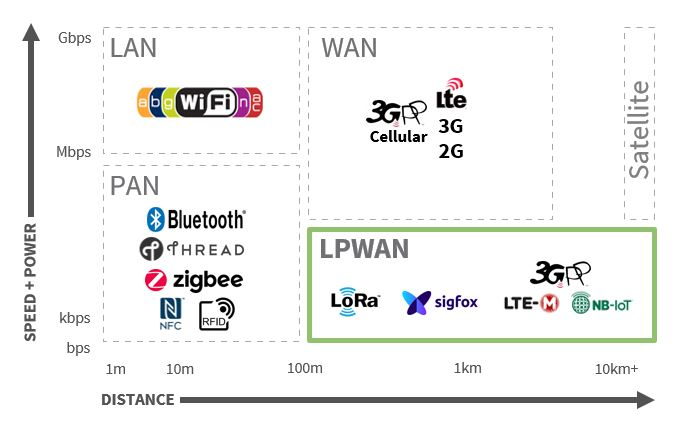
\includegraphics[width=0.6\linewidth]{figuras/iotprotocols.jpg}
        \caption*{\small{Fonte: iot.do, 2021}}
    \end{figure}   

\end{frame}


\begin{frame}{Elementos Base}{O protocolo MQTT}

    \begin{itemize}
        \item \textbf{\textit{Message Queuing Telemetry Transport}} - MQTT foi inventado e desenvolvido inicialmente pela \textit{International Business Machines} - IBM;
        \item É um protocolo de mensagem com suporte para a comunicação \textbf{assíncrona} entre as partes;
        \item Projetado para aplicações que utilizam pouca banda de rede utilizando um modelo de publicação e assinatura;

    \end{itemize}


\end{frame}

\begin{frame}{Elementos Base}{O protocolo MQTT}

    \begin{itemize}
        \item Em uma rede MQTT existem dois agentes principais: o \textit{\textbf{broker}} e os \textit{\textbf{clients}};
        \item O \textit{broker} é um servidor que centraliza as mensagens dos clientes e as encaminha para os clientes interessados;
        \item É um dispositivo ou serviço que tenha capacidade de interagir com o \textit{broker} e trocar mensagens;

    \end{itemize}


\end{frame}

\begin{frame}{Elementos Base}{O protocolo MQTT}

    \begin{figure}[H]
        \centering
        \caption{Diagrama básico MQTT}
        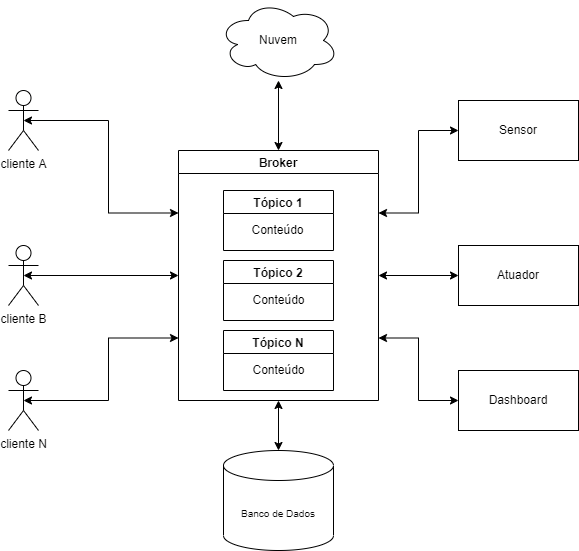
\includegraphics[width=0.45\textwidth]{figuras/mqtt.drawio.png}
        \caption*{\small{Fonte: própria, 2021}}
        \label{fig:mqtt_diagram}
    \end{figure}

\end{frame}

\begin{frame}{Elementos Base}{O protocolo MQTT}
    \begin{itemize}
        \item Como qualquer outro protocolo de comunicação o MQTT possui diversos termos e características associadas, como a segurança, a definição dos \textit{endpoints}\footnote{\textbf{endpoints} - Pontos de extremidade. Terminais de conexão entre uma API e o cliente.}, o endereçamento, tipo de dado trafegado, entre outros.
    \end{itemize}

\end{frame}

\begin{frame}{Elementos Base}{O protocolo MQTT}
    \begin{itemize}
        \item \textbf{\textit{broker}}: É o intermediário no processo de comunicação, atuando como um servidor;
        \item \textbf{\textit{client}}: Responsável por estabelecer e manter uma conexão com o \textit{broker}, enviar e receber as mensagens;
        \item \textit{\textbf{broker ip}}: Identificação única do servidor \textit{\textbf{broker}} conectado em determinada rede;
        \item \textbf{\textit{broker username e broker password}}: Credenciais, opcionais, para determinado cliente estabelecer conexão com o servidor; 
    \end{itemize}

\end{frame}

\begin{frame}{Elementos Base}{O protocolo MQTT}
    \begin{itemize}
        \item  \textit{\textbf{QoS}}: Nível de qualidade do serviço desejado, indicando como deve ser a relação entre os elementos comunicantes.\cite{fabiobrandao};
        \item \textbf{\textit{last good message}}: É a operação à qual o \textit{broker} envia a última menagem válida recebida em um determinado tópico ao ser requisitado por um cliente;
        \item \textbf{\textit{last will testament (LWT)}}: São mensagens pré-definidas a serem publicadas pelo broker em nome de um determinado cliente, uma vez que esse cliente está \textit{offline} e não pode publicar mais;
        \item \textbf{\textit{keep alive}}: Mensagens periódicas enviadas por determinado cliente buscando validar a conexão;
    \end{itemize}

\end{frame}

\begin{frame}{Elementos Base}{O protocolo MQTT}
    \begin{itemize}
        \item \textbf{tópicos, \textit{publish} e \textit{subscribe}}: O ato de um cliente enviar uma mensagem é chamado \textit{publish}(publicação). E para receber mensagens de determinado um tópico um cliente deve fazer um \textit{subscribe}(inscrição). Os níveis de um tópico são separados por “/” e um cliente pode optar por se inscrever em quantos tópicos forem necessários, utilizando os artifícios da \autoref{tab:simbolos_mqtt}.
    \end{itemize}

\end{frame}

\begin{frame}{Elementos Base}{O protocolo MQTT}
    \begin{table}[H]
        \centering
        \resizebox{\textwidth}{!}{%
            \begin{tabular}{c|c|c}
                \hline
                Símbolos & Descrição & Exemplo \\ \hline
                + & Retorna ou envia qualquer informação naquele nível (Coringa) & \begin{tabular}[c]{@{}c@{}}area/10/sensor/5000/temperatura\\ area/10/sensor/4000/temperatura\\ area/10/sensor/+/temperatura\end{tabular} \\ \hline
                \# & Retorna ou envia qualquer coisa abaixo daquele nível & area/10/\# \\ \hline
                \$ & Tópicos iniciados com \$ são especiais usados internamente pelo broker. & \$SYS/broker/clients/total \\ \hline
            \end{tabular}%
        }
        \caption{Caracteres especiais utilizados para envio e recebimento no protocolo MQTT.}
        \label{tab:simbolos_mqtt}
    \end{table}

\end{frame}


\begin{frame}{Fundamentação Teórica}{Elementos de \textit{Hardware}}
\end{frame}

\begin{frame}{Fundamentação Teórica}{Elementos de \textit{Firmware}}
\end{frame}

\begin{frame}{Fundamentação Teórica}{Elementos de \textit{Software}}
\end{frame}

\section{Metodologia}
\begin{frame}{Metodologia}
\begin{columns}[c] % The "c" option specifies centered vertical alignment while the "t" option is used for top vertical alignment

\column{.45\textwidth} % Left column and width
\textbf{Passos da metodologia}
\begin{enumerate}
\item Statement
\item Explanation
\item Example
\end{enumerate}

\column{.5\textwidth} % Right column and width
Explicando alguma coisa ... lorem ipsum dolor sit amet, consectetur adipiscing elit. Integer lectus nisl, ultricies in feugiat rutrum, porttitor sit amet augue. Aliquam ut tortor mauris. Sed volutpat ante purus, quis accumsan dolor.

\end{columns}
\end{frame}

\section{Resultados}
\begin{frame}{Resultados}
\begin{table}
\begin{tabular}{l l l}
\toprule
\textbf{Treatments} & \textbf{Response 1} & \textbf{Response 2}\\
\midrule
Treatment 1 & 0.0003262 & 0.562 \\
Treatment 2 & 0.0015681 & 0.910 \\
Treatment 3 & 0.0009271 & 0.296 \\
\bottomrule
\end{tabular}
\caption{Table caption}
\end{table}
\end{frame}

\begin{frame}{Resultados}
    
\begin{figure}
    \centering
    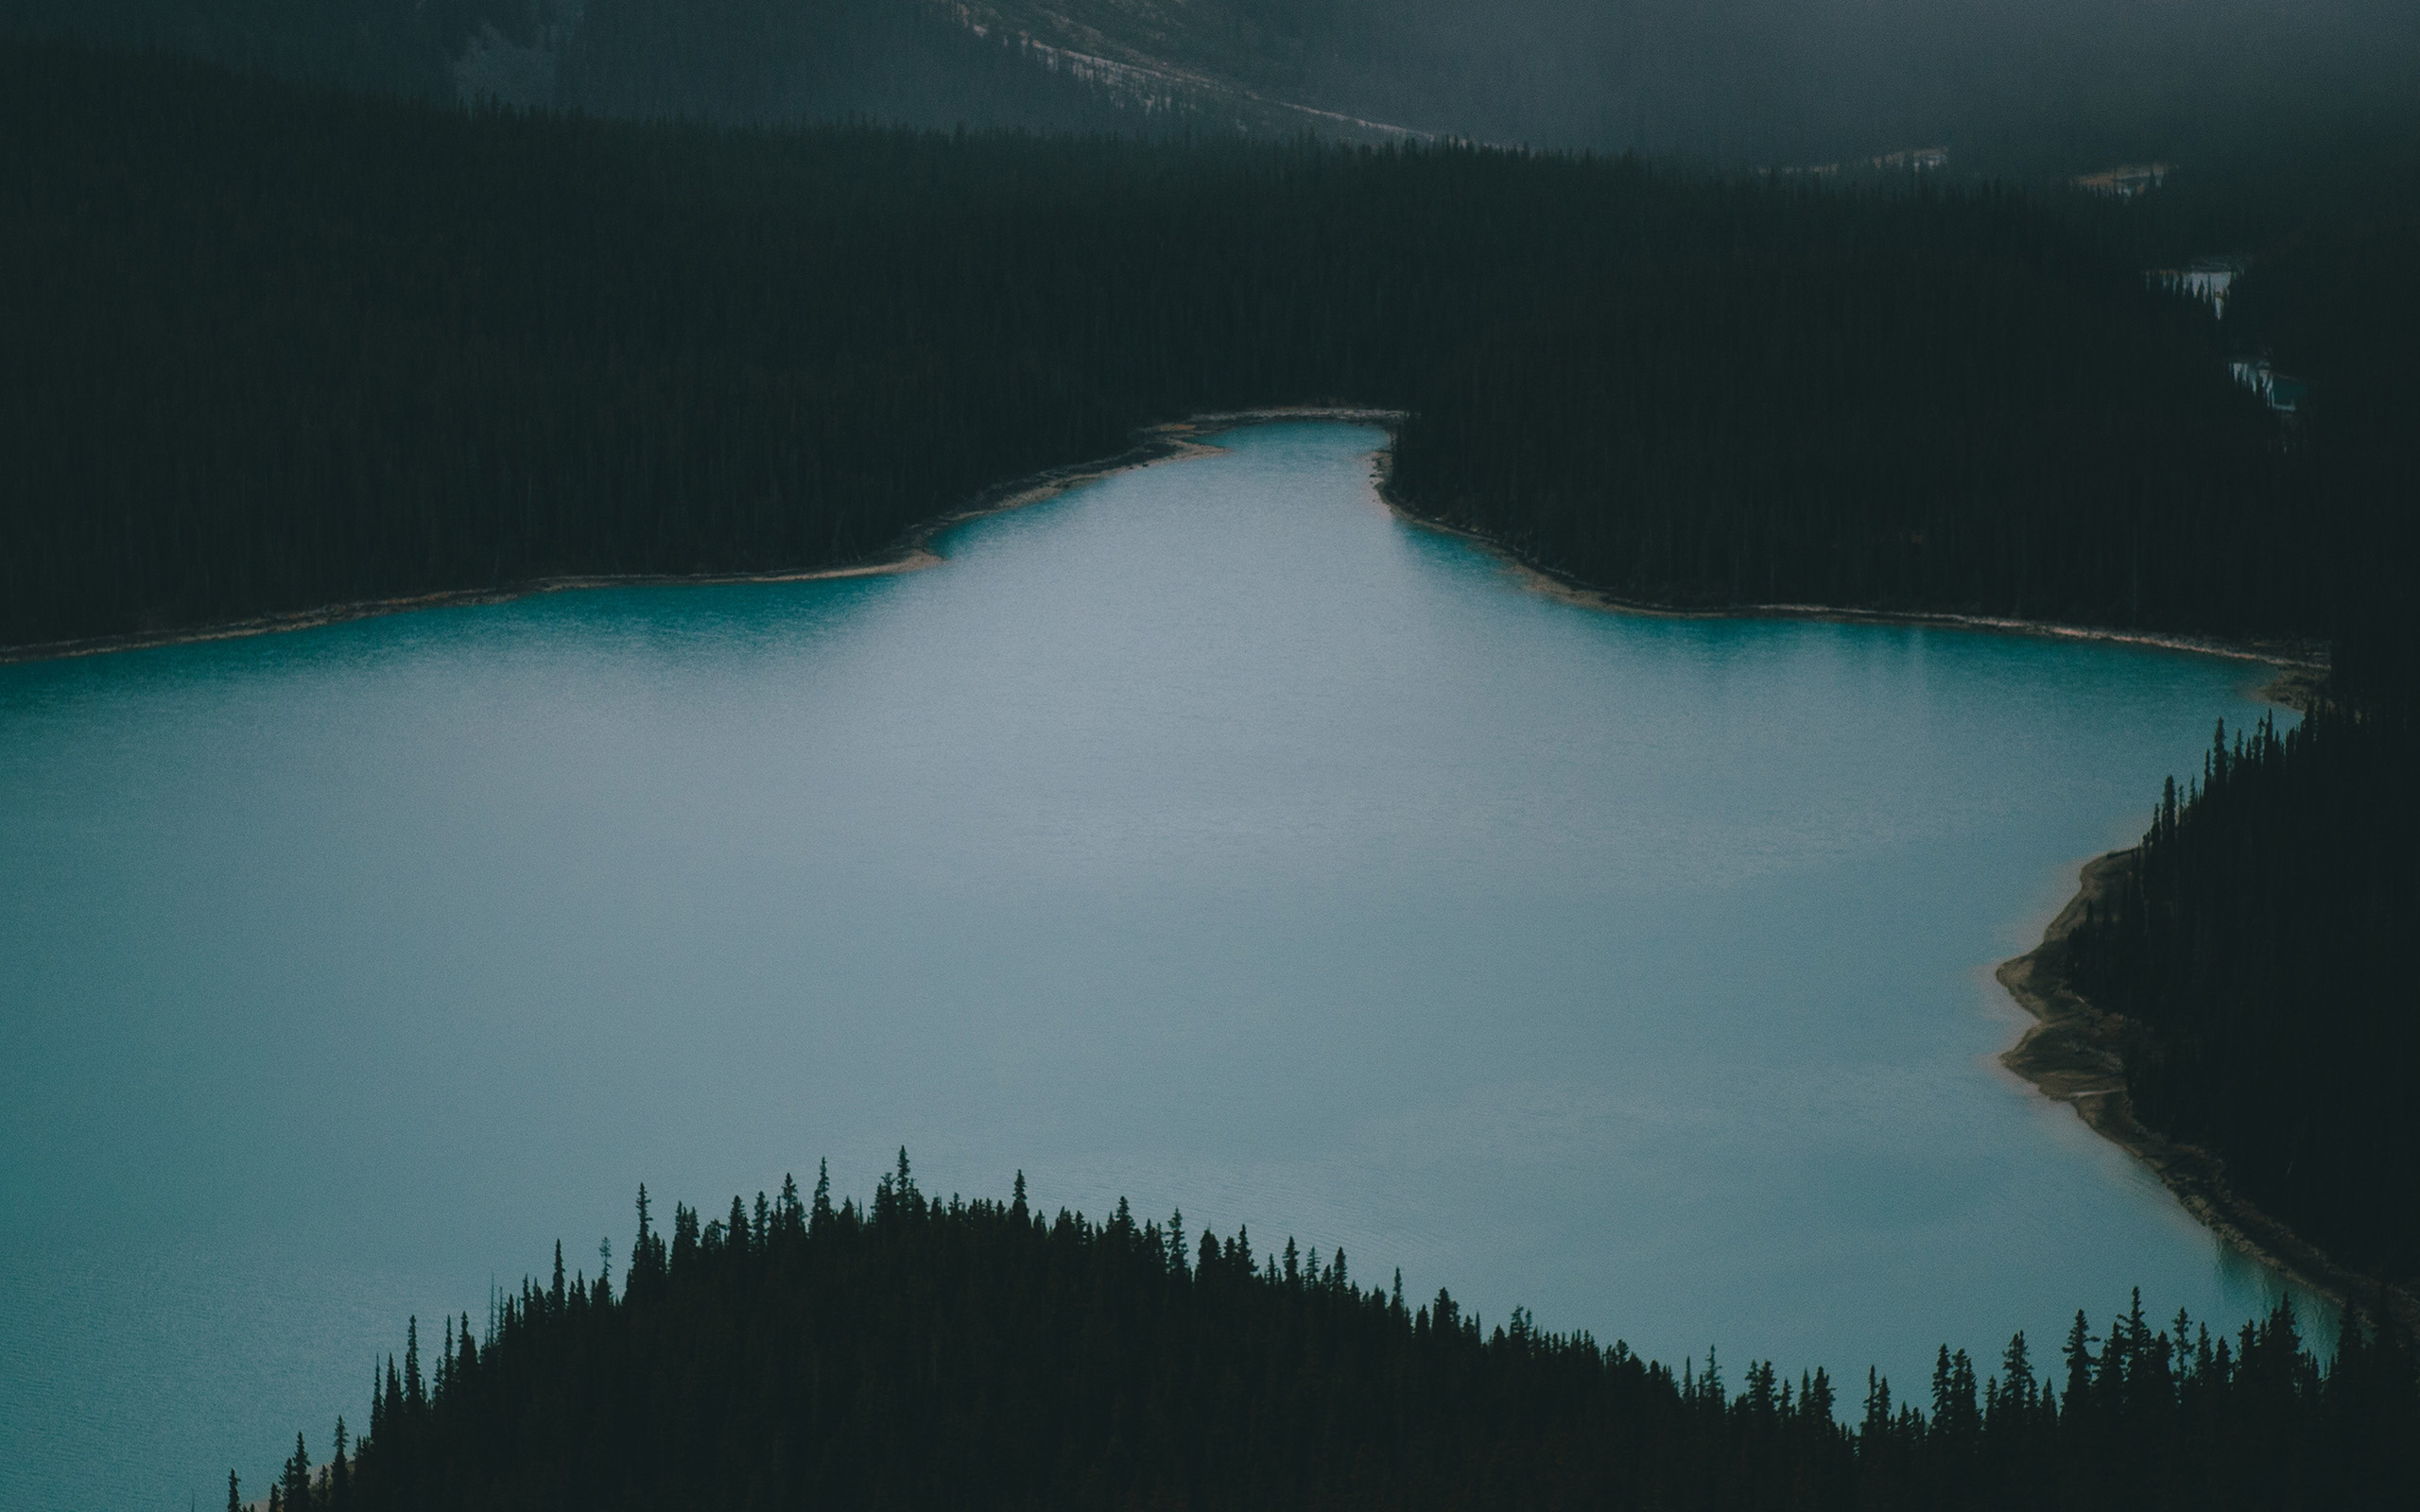
\includegraphics[width=.7\textwidth]{img/river.jpg}
    \caption{Aqui temos a imagem de um lago}
    % \label{fig:my_label}
\end{figure}

\end{frame}

\section{Conclusão}
\begin{frame}{Conclusão}
\begin{itemize}
\item more work
\medskip
\item more responsibility
\medskip
\item more satisfaction
\end{itemize}
    
\end{frame}


%%%%%%%% agradecimentos %%%%%%%%
\begin{frame}{Agradecimentos}
    \large{Agradeço a fulano, ciclano e beltrano que apoiaram o desenvolvimento dessa pesquisa.}
\end{frame}
%------------------------------------------------


%------------------------------------------------
%------------------------------------------------
%%%%%%%% referencias %%%%%%%%
%\nocite{*}
\begin{frame}[allowframebreaks]{Referências}
\bibliographystyle{unsrt}
\bibliography{base-referencias}
\end{frame}


%%%%%%%% repete primeiro slide %%%%%%%%
\begin{frame}
\titlepage 
\end{frame}


\end{document}